\documentclass{article}
\usepackage[margin=1in]{geometry} 
\usepackage{amsmath}
\usepackage[T1]{fontenc}          % change font encoding to T1
\usepackage{lmodern}  %better for visual on screen
\usepackage{graphicx}
\usepackage{float}
\usepackage{enumitem}
\usepackage{mathtools}
\usepackage{booktabs}
\usepackage{dirtree}

\makeatletter
\renewcommand*\env@matrix[1][\arraystretch]{%
	\edef\arraystretch{#1}%
	\hskip -\arraycolsep
	\let\@ifnextchar\new@ifnextchar
	\array{*\c@MaxMatrixCols c}}
\makeatother

% Used for adding Matlab Algorithms
\RequirePackage{listings}
\RequirePackage[framed,numbered]{matlab-prettifier}

\DeclarePairedDelimiter\abs{\lvert}{\rvert}%

\begin{document}
\section{roundgridfun.m}
\lstinputlisting[
label      = {alg:lsr},
style      = Matlab-editor,
basicstyle = \mlttfamily,
firstline  = 1,
lastline   = 33,
firstnumber= 1
]{../roundgridfun.m}

\subsection{Motivation/Concept}
This function was created as a fast way to grid dense data in Matlab using a nearest neighbor binning technique.  Often when gridding high density data to a lower density grid, a Delaunay Triangulation does not make sense as your just effectively down-sampling your dataset, and an IDW, while certainly a more elegant and accurate solution, can sometimes be fairly time consuming in matlab.  Additionally, \textit{roundgridfun.m} works on N-D datasets and has the ability for alternative function handles to be passed in, which can be used to do more than just calculate the mean of the points in a bin.

\clearpage
\subsection{Math}
The input for the algorithm is the raw data, the grid nodes, and the function handle to operate on each computed bin.  The algorithm computes which points lie in the bin associated with each grid node, and uses the function handle to compute a value for each bin.  Note, to improve processing time, roundgridfun is written with the assumption that the grid spacing along each dimension is constant.

The data is converted from the raw coordinate system to an index based coordinate system based on the grid.  The data is then rounded (hence, roundgridfun) to determine the associated grid node that each raw data point should be mapped to.  Data that is mapped to a bin that is not associated with a grid node is omitted from the results.  

A conceptual diagram of the algorithm for gridding 3D data onto a 2D Grid is shown below:
\begin{figure}[H]
	\centering
	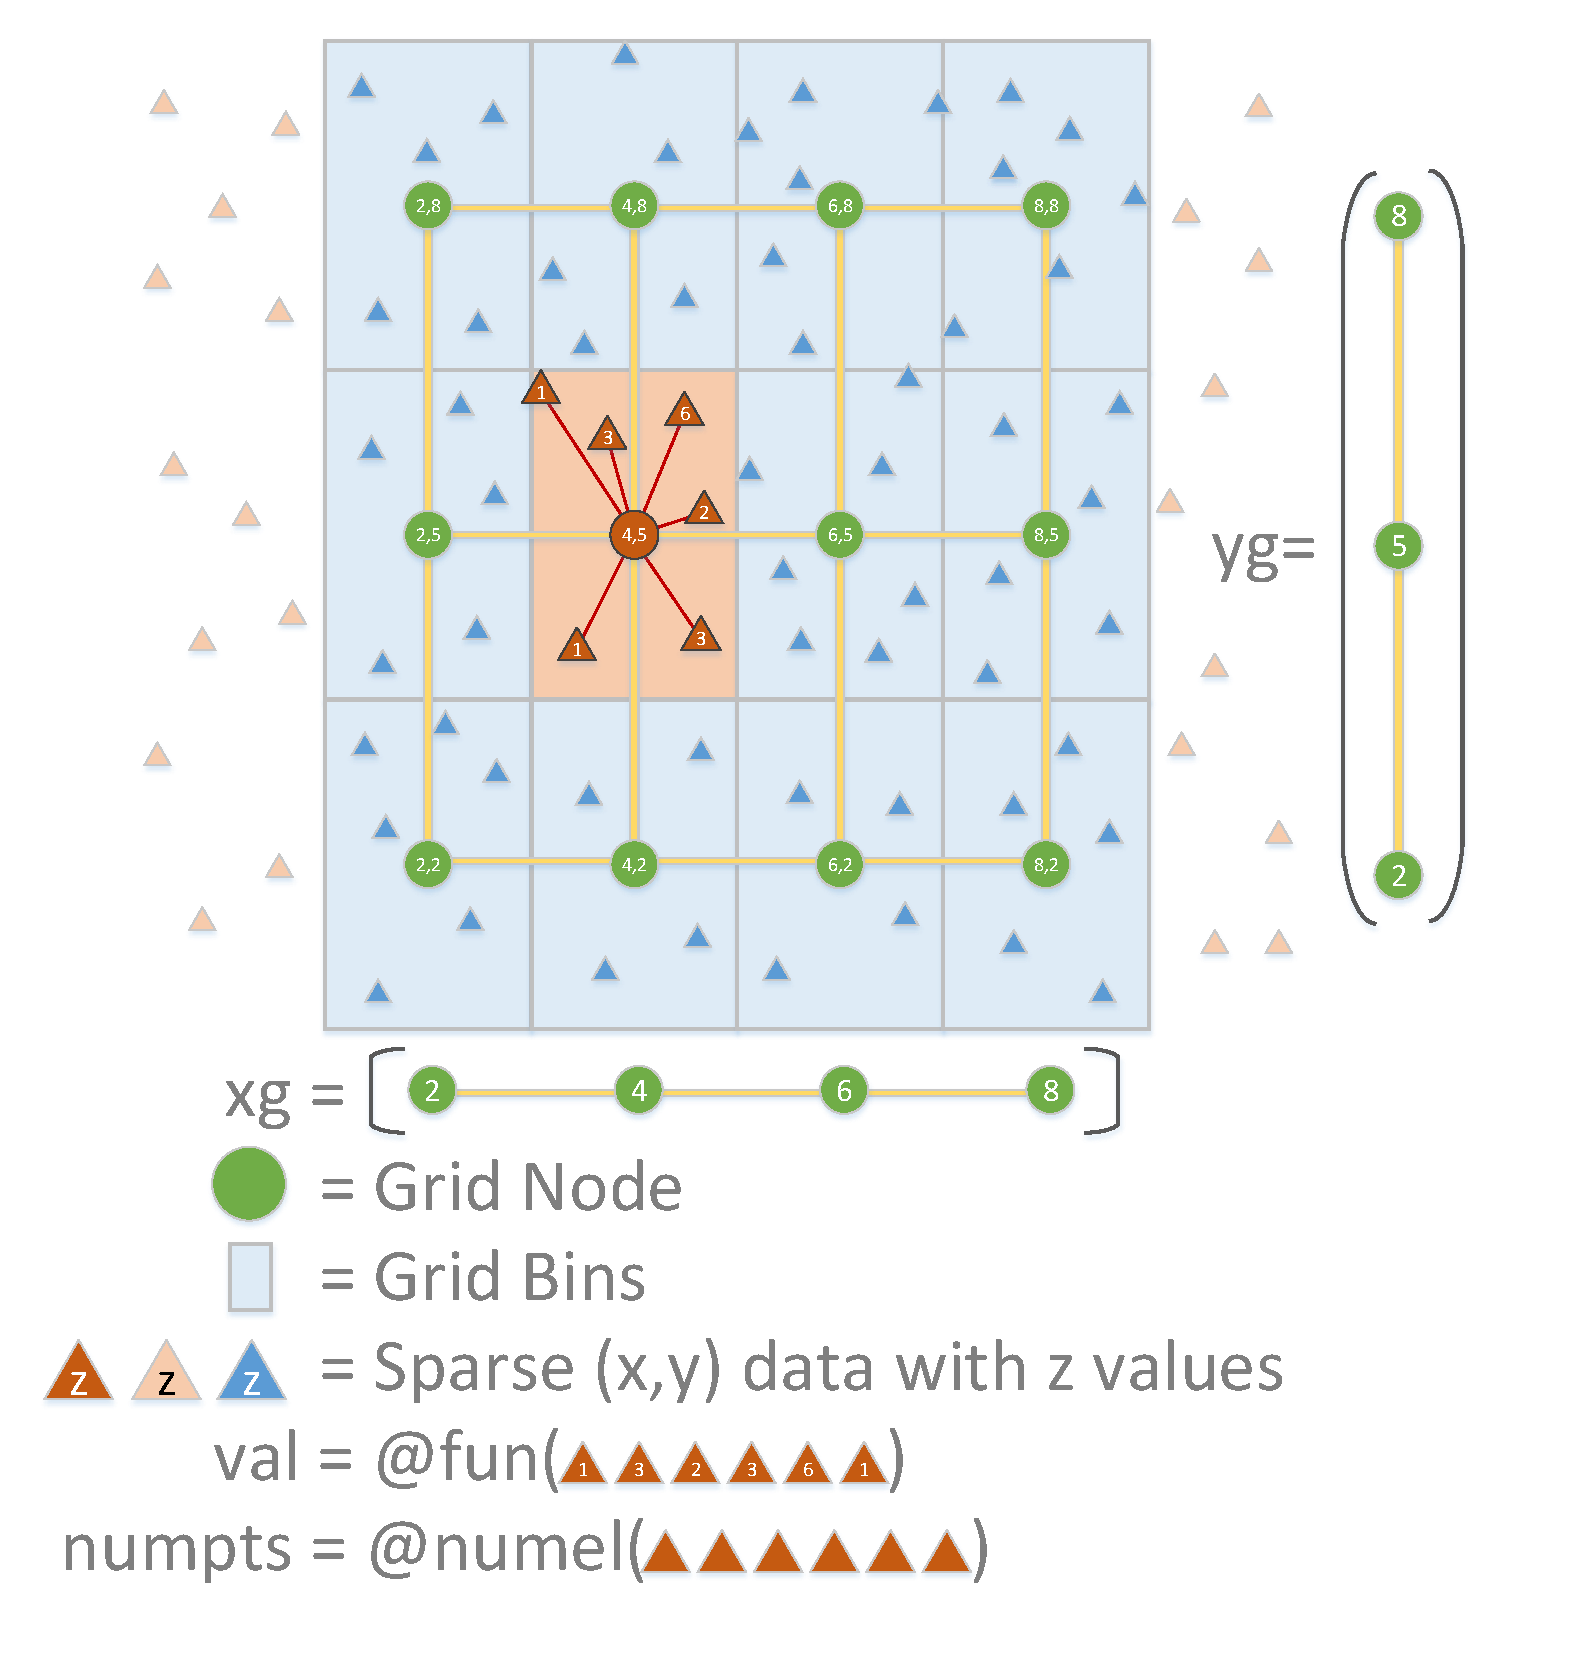
\includegraphics[width = \linewidth]{roundgridfunmaplabels}
\end{figure}

\subsection{Inputs}
\subsubsection{x}
vector of x data points

\subsubsection{y}
vector of y data points

\subsubsection{z}
vector of z data points

\subsubsection{xg}
Either a vector of x grid nodes, or a meshgrid 2d array of x grid nodes

\subsubsection{yg}
Either a vector of y grid nodes, or a meshgrid 2d array of y grid nodes

\subsubsection{fun}
Function handle which inputs a vector of x, and outputs a single value

eg. @mean, @min, @std, @max, @var, @(x) {x}

\subsection{Outputs}
\subsubsection{val}
Value from @fun computed for each grid node

\subsubsection{numpts}
Number of points in each grid node

\clearpage
\subsection{Examples \textit{exampleRoundgridfun.m}}
\subsubsection*{2D Case (@mean)}
This example demonstrates gridding 2D (x,y) data onto an x grid using the mean values in each grid bin.
\lstinputlisting[
label      = {alg:lsr},
style      = Matlab-editor,
basicstyle = \mlttfamily,
firstline  = 3,
lastline   = 9,
firstnumber= 3
]{../exampleRoundgridfun.m}

\begin{figure}[H]
	\centering
	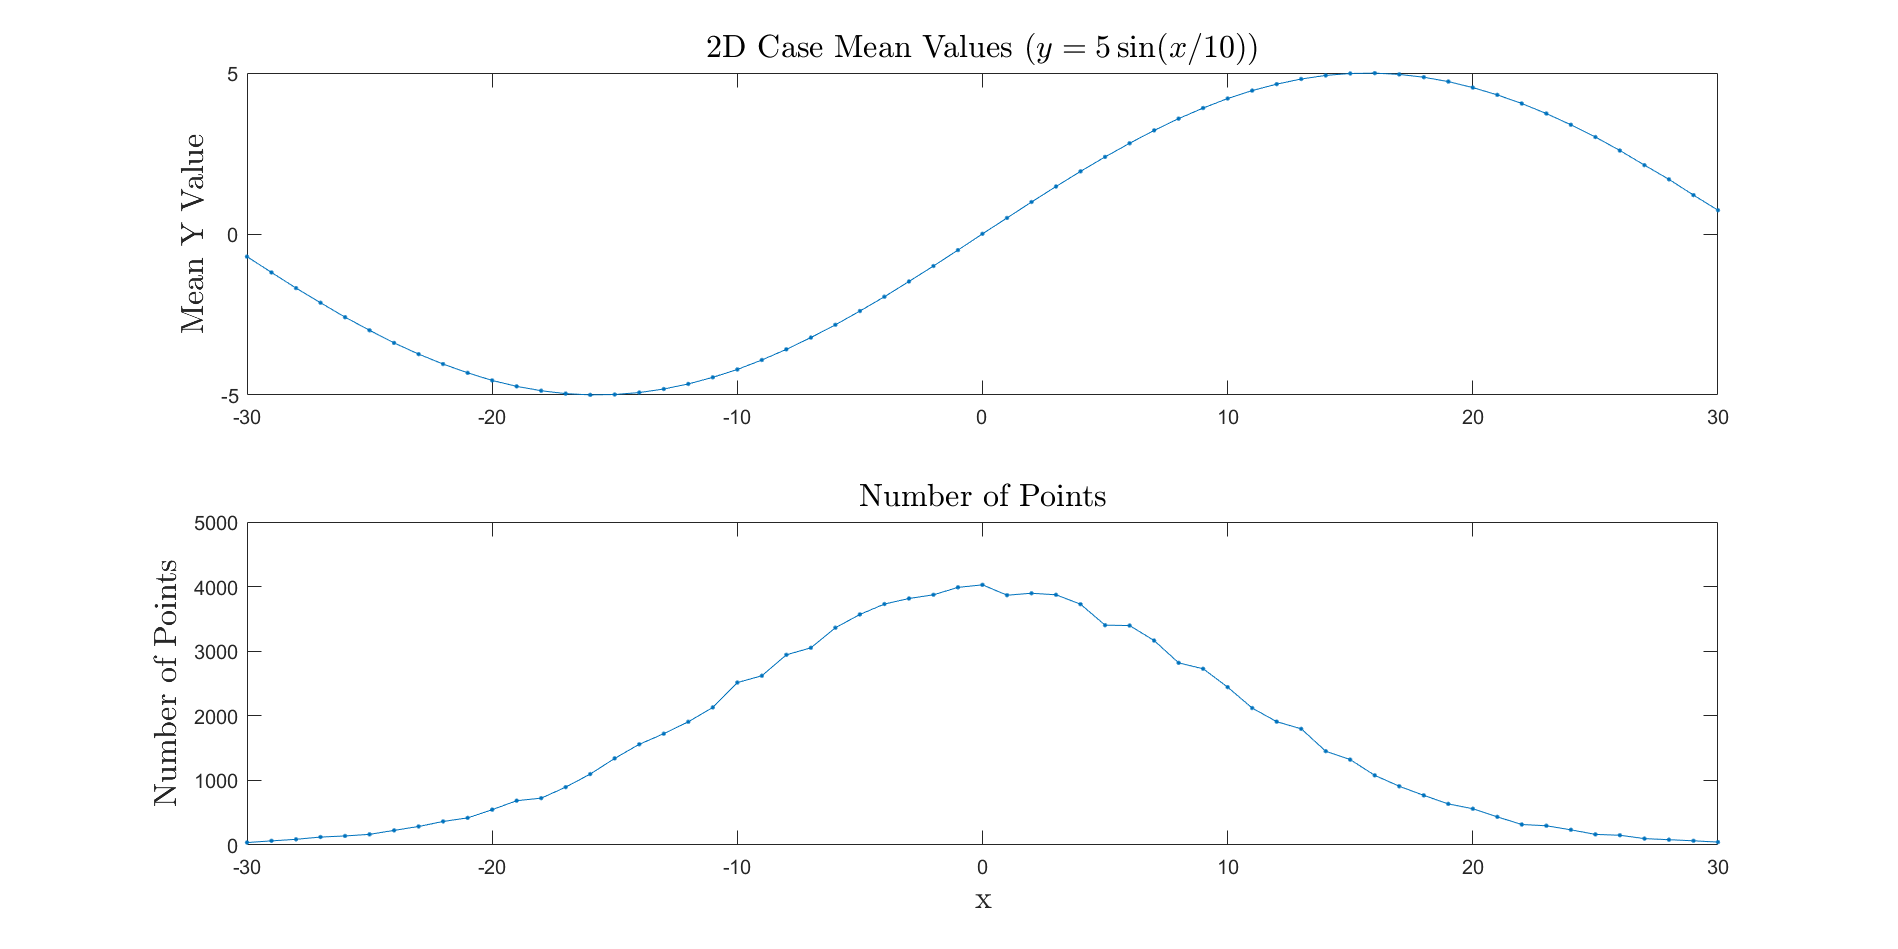
\includegraphics[width = \linewidth]{2d}
\end{figure}

\clearpage
\subsubsection*{2D Case (cell array)}
This example demonstrates how all of the y values in each bin can be returned by returning a cell from the function input.  Here, the y values in each bin are sorted, and assembled in a 2D matrix for visualization.
\lstinputlisting[
label      = {alg:lsr},
style      = Matlab-editor,
basicstyle = \mlttfamily,
firstline  = 24,
lastline   = 37,
firstnumber= 24
]{../exampleRoundgridfun.m}

\begin{figure}[H]
	\centering
	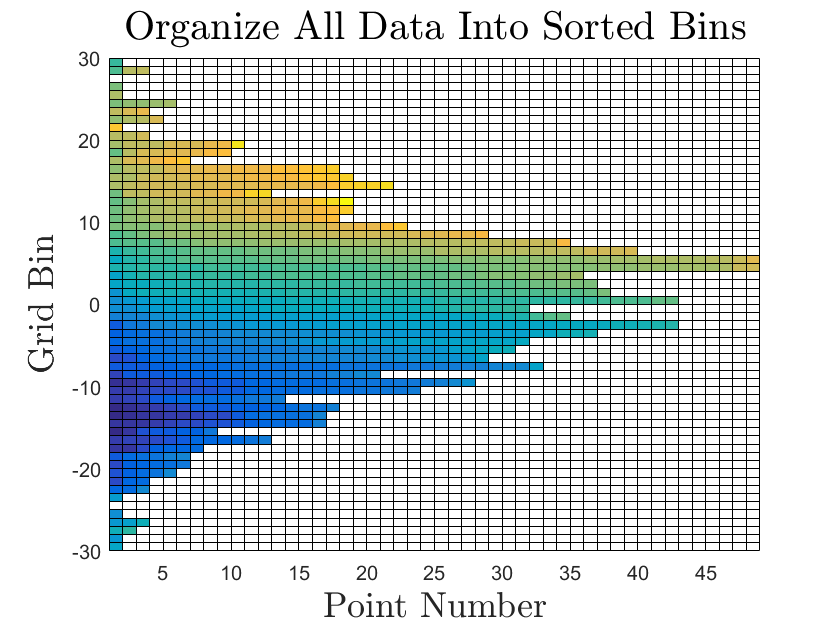
\includegraphics[width = \linewidth]{2dbins}
\end{figure}

\clearpage
\subsubsection*{3D Case (@min)}
This examples grids 3D data using the min of all of the data in each bin.
\lstinputlisting[
label      = {alg:lsr},
style      = Matlab-editor,
basicstyle = \mlttfamily,
firstline  = 43,
lastline   = 50,
firstnumber= 43
]{../exampleRoundgridfun.m}

\begin{figure}[H]
	\centering
	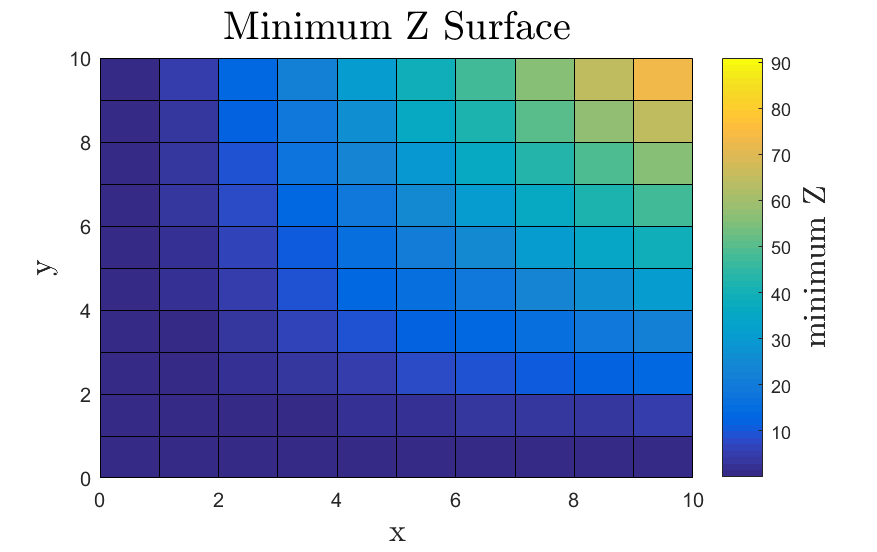
\includegraphics[width = \linewidth]{3d}
\end{figure}

\clearpage
\subsubsection*{4D Case (@mean)}
This example demonstrates the creation of rectangular prism voxels.  
\lstinputlisting[
label      = {alg:lsr},
style      = Matlab-editor,
basicstyle = \mlttfamily,
firstline  = 62,
lastline   = 71,
firstnumber= 62
]{../exampleRoundgridfun.m}

\begin{figure}[H]
	\centering
	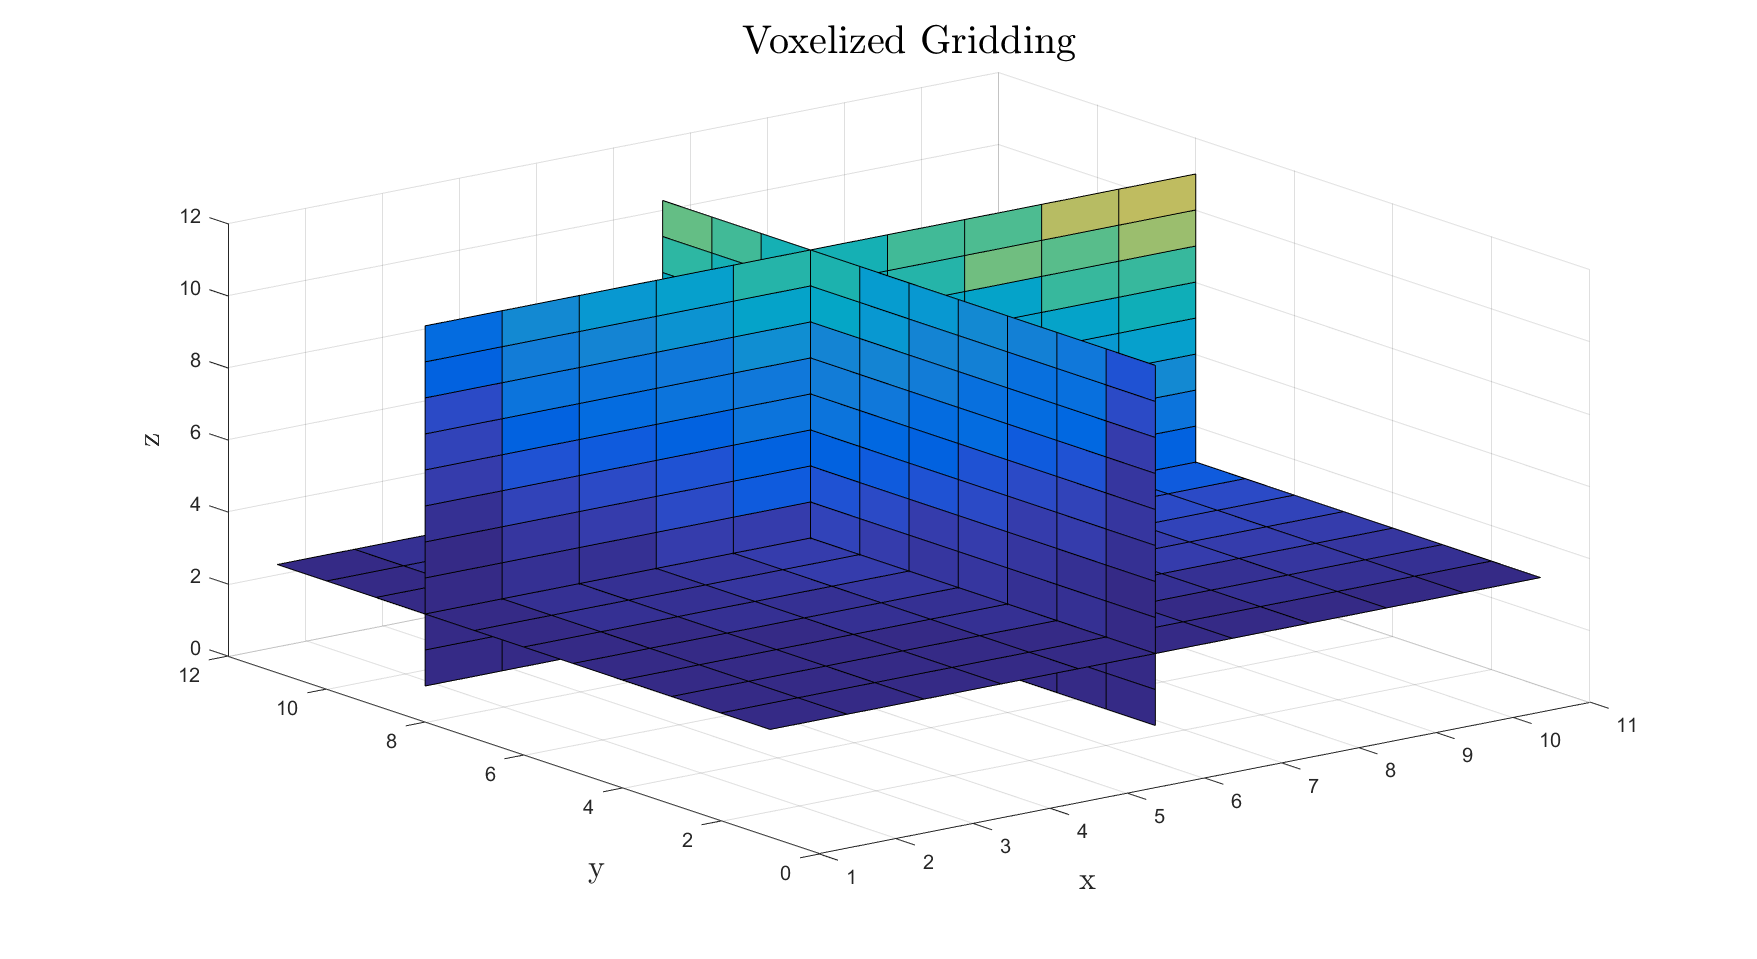
\includegraphics[width = \linewidth]{4d}
\end{figure}

\clearpage
\subsubsection*{5D Case (@std)}
This example demonstrates how higher order data can also be gridded into higher dimensions.
\lstinputlisting[
label      = {alg:lsr},
style      = Matlab-editor,
basicstyle = \mlttfamily,
firstline  = 79,
lastline   = 85,
firstnumber= 79
]{../exampleRoundgridfun.m}

\begin{figure}[H]
	\centering
	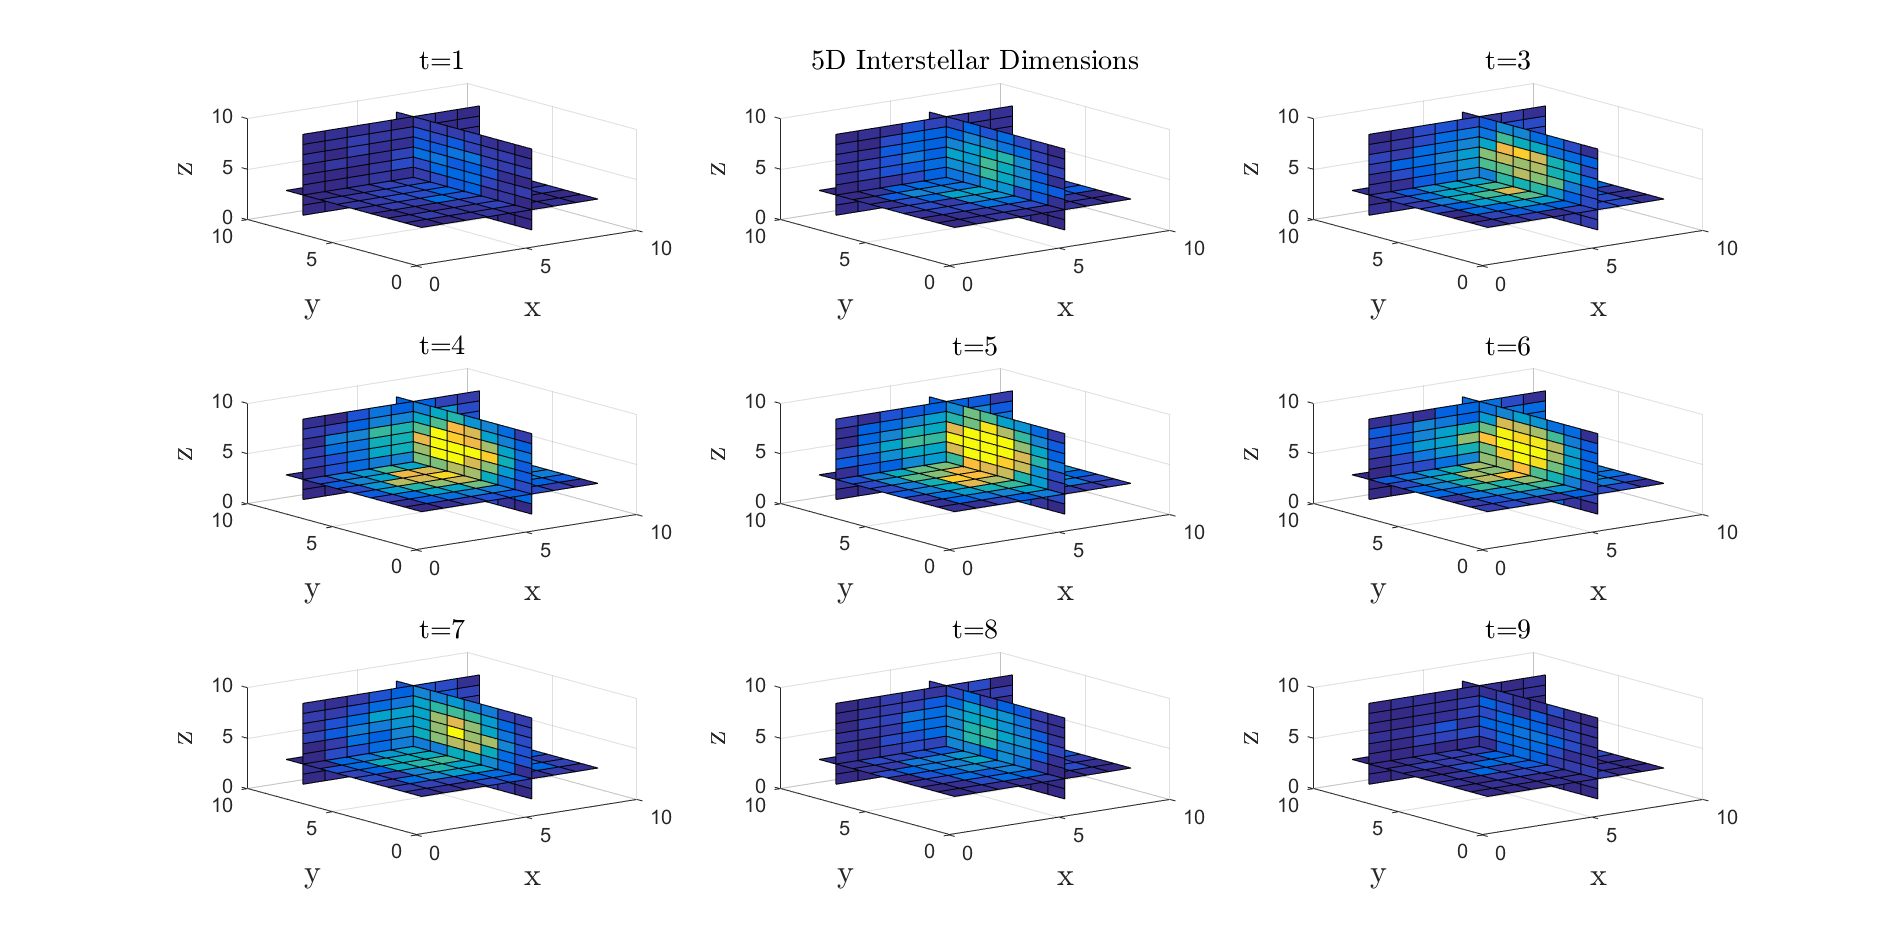
\includegraphics[width = \linewidth]{5d}
\end{figure}

\end{document}